\chapter{Inventing Color}

Everything glows (gives off electromagnetic radiation) when it has a temperature --- particles are wiggling around randomly (faster if it's hotter) and giving off energy as they wiggle. This \textbf{thermal radiation}, also called blackbody radiation, is the same for any object at the same temperature. This means we can take something's temperature by looking at the spectrum of light it gives off. This is great for learning about something's temperature at a distance, like stars.

Incandescent lightbulbs are so warm that they glow in the visible spectrum (like stars). In this lab, you'll investigate the radiation that is given off by a lightbulb at various temperatures, then use filters to mimic the situation astronomers are in when they observe astronomical objects with different color filters. You'll invent a metric to numerically state the temperature of the lightbulb, even without knowing the actual temperature. Finally, you'll use the various images that you took with SEO with different color filters and combine them to form a color image.

\section{Lightbulbs}

\begin{steps}
	\item Using the spectrometer, observe the spectrum created by a lightbulb at various brightnesses / voltages.  What's the overall shape? How does the shape change when the brightness increases? How does the peak frequency change? How does the visual color of the bulb change as it gets brighter? As the lightbulb gets brighter, the filament inside gets hotter. If all objects act like the tungsten filament as it gets hotter, what general pattern can you state about the EM radiation given off by an object as a function of its temperature?

\end{steps}

Cameras have come a long way since the days of developing film, but sensors are not as smart you might think. They register light, but they can't usually tell the color (i.e. wavelength) of the incoming photons. So then how do you get a color image? In astronomy (and in your cell phone!) color images are generated by measuring the amount of light at specific colors and then combining these measurements to create a colorful image. A filter is used to select bands of color to allow through. In consumer cameras and phone cameras, these filters are permanently attached to the front of individual pixels. In astronomical imaging, there is no permanent filter, and different filters are moved into place.

\begin{steps}
	\item Use the red and green filters in front of the fiber optic input to the spectrometer to see how they affect the spectrum that is received. \textbf{Save a graph of the spectrum with each filter and include in your report.}
\end{steps}

In a regular astronomical image, each pixel gives just one value --- the number of counts detected in that pixel, regardless of the wavelength of the photon detected. We can treat the fiber optic as a single-pixel camera if we count up the total number of counts detected. To find that total number, you can find the area under the curve in the plot.

\begin{steps}
	\item With no filter, add up the total number of counts detected by calculating the area under the curve. To do this in an approximate way, count the number of boxes underneath the curve, then multiply this by the height of one box (in counts per nanometer) and by the width of one box (in nanometers).
	
	\item Do the same for the spectrum using the red and green filters separately.
\end{steps}

Now you have the value of our single-pixel camera for the case of clear (no filter), red, and green filters. Time to revisit the pattern found above in Step 1.

\begin{steps}
	\item If that pattern from Step 1 is true, what should happen to the relative values of red and green as the voltage is increased? Should one increase more than the other?
	
	\item Perform an experiment to test whether this prediction is supported.
\end{steps}

\section{Creating a color image}

Now you'll create a color image from the three images you took last week, of the same target with r, g, and b filters.

\textbf{Loading and manipulating images in ds9 consists of:}
\begin{itemize}
\item loading an image  (file > open)
\item setting z1,z2 on an image  (scale > various algorithms; use scale > scale parameters for full control). See Figures \ref{ic:fig:z-min-max}--\ref{ic:fig:z-small} for examples.
\item controlling the intensity mapping within those bounds (mouse right click-and-hold and drag)
\end{itemize}

\begin{figure}
	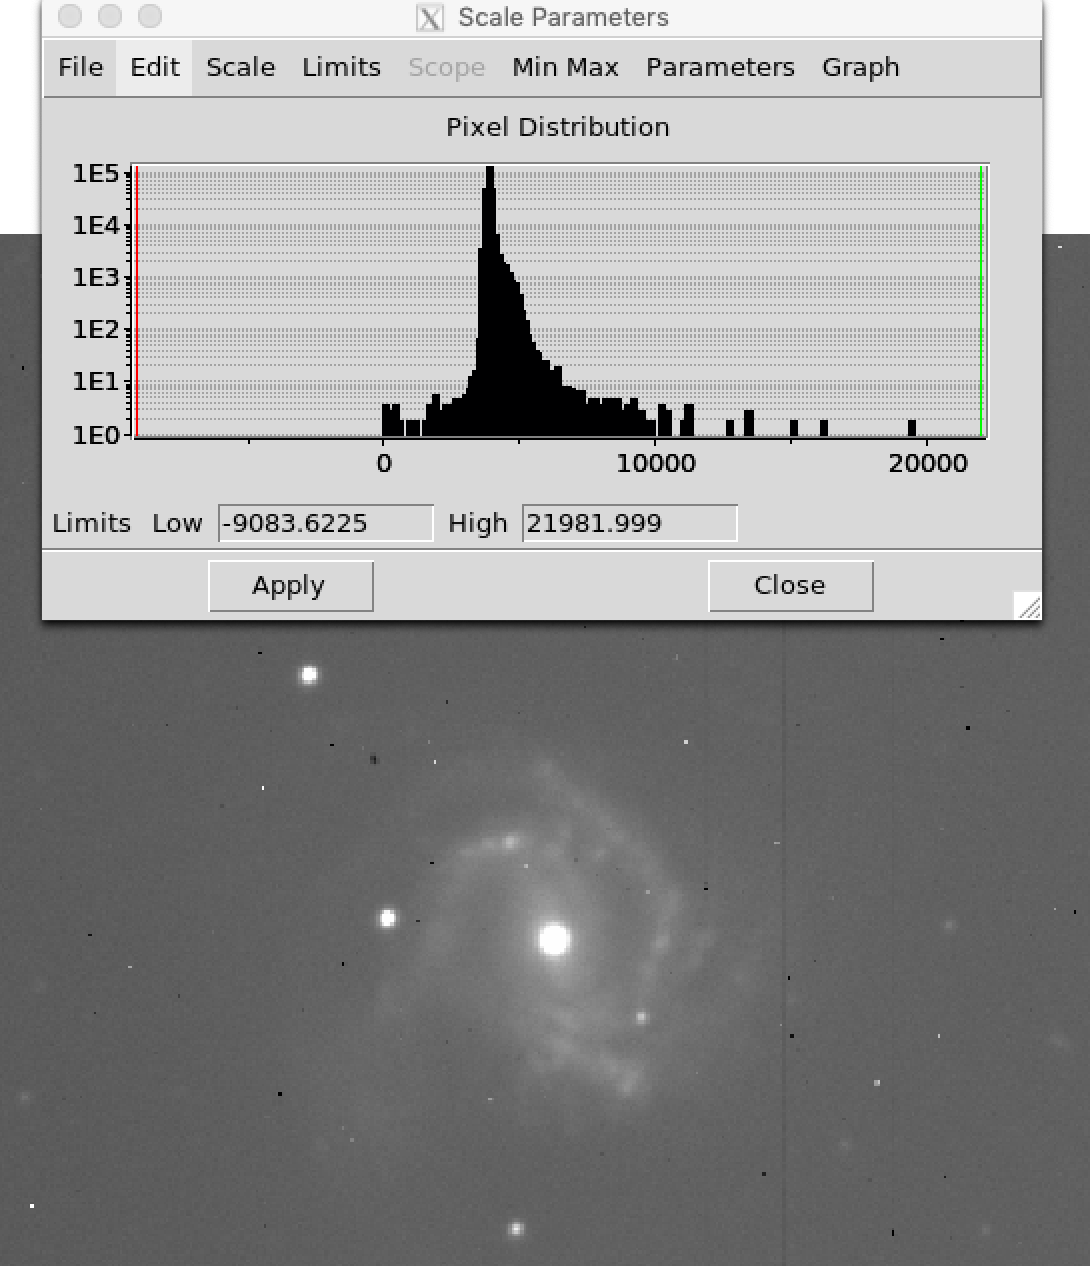
\includegraphics[width=0.5\textwidth]{inventing-color/z-min-max}
	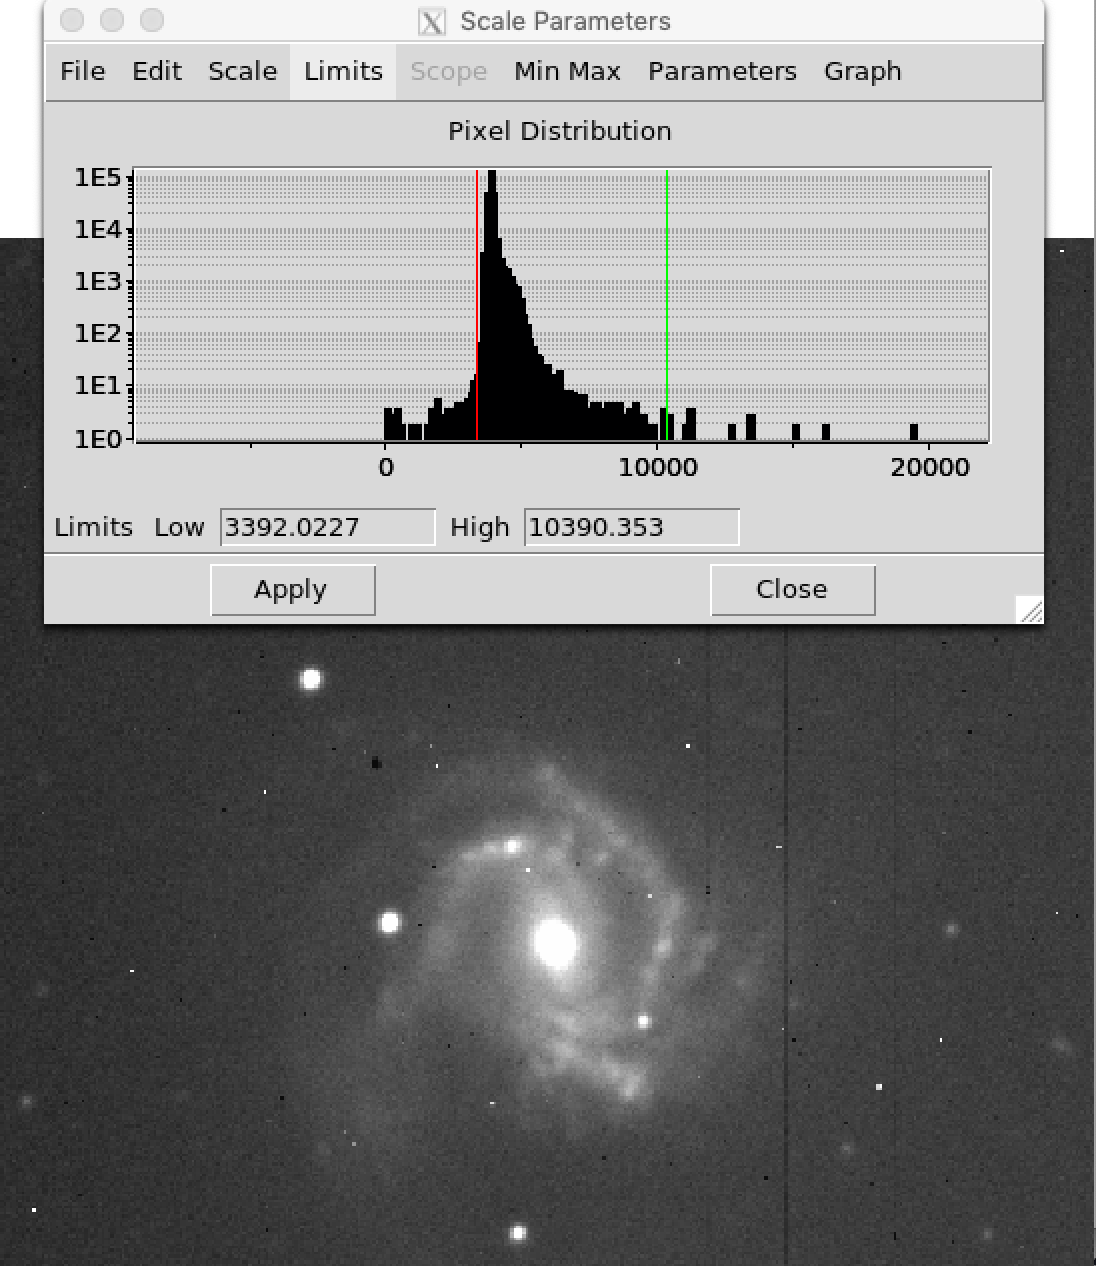
\includegraphics[width=0.5\textwidth]{inventing-color/z-mid}
	\caption{Proper choice of data ranges is important. The default for ds9 is often the min/max values in the image, which can be a poor choice if there are outlier pixels, as shown here on the left. The red line shows the lower limit z1, which is mapped to no color (black here), and the green line is the upper limit z2, mapped to full color (white here). Pixel values between these are shown in various brightnesses of the color. On the right, z1 and z2 are more tuned to the distribution of pixel values, which more effectively uses the dynamic range of the display for pixel values where there are significant amounts of data.}\label{ic:fig:z-min-max}
\end{figure}

\begin{figure}
		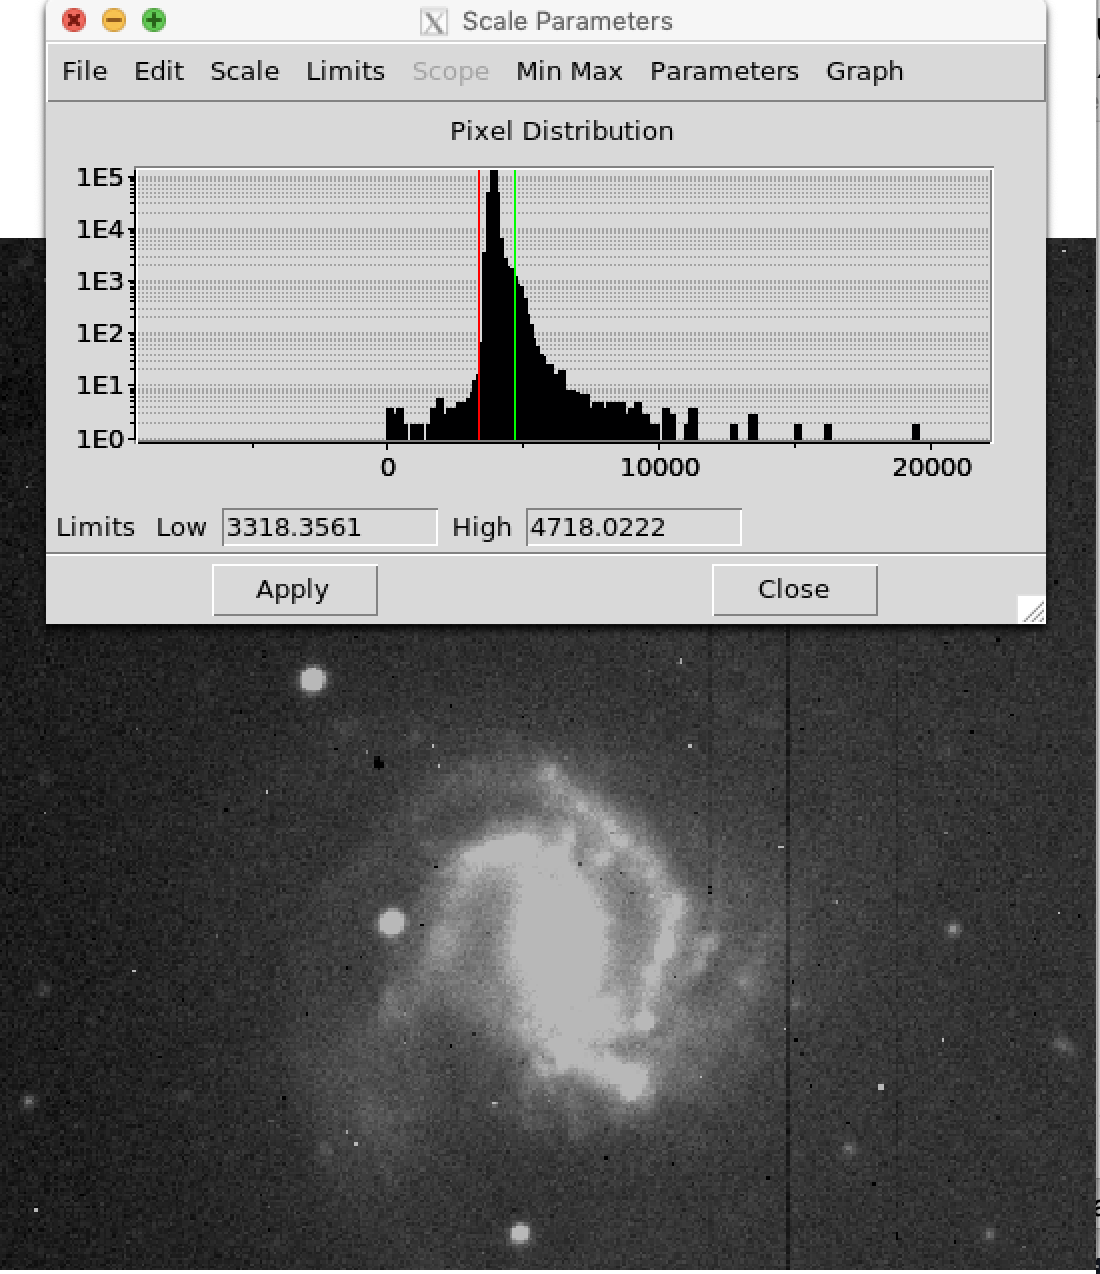
\includegraphics[width=0.5\textwidth]{inventing-color/z-small}
		\caption{Smaller values of z2 will emphasize fainter values in the target. Compare the image to the left to the right-hand image above.}\label{ic:fig:z-small}
\end{figure}

\textbf{You can change the zoom and center location in an image by} 
\begin{itemize}
\item moving around in image (mouse middle click if edit>point is set[the default], or edit>pan and mouse left click)
\item zooming in and out (mouse wheel, zoom> +,- etc.)
\end{itemize}

\textbf{To build a color image}
\begin{itemize}
\item Open a color (rather than monochrome) frame:  Frame > new rgb
\item Open the red, green, blue files using the rgb subwindow to select which channel you are working in, and then scale and control intensities on each one. 
\item There are many possible ways to scale the images. Some testing suggests that choosing Scale > ASINH (or Linear or Square Root as other choices) and Scale > 99.5\% (or maybe 99\% or 98\%)  produces reasonable results. Experiment!
\item One thing to note: the rgb subwindow allows you to control how the images are aligned spatially via the “align” menu at the top. There are three relevant choices: “WCS”, “Image” or “Physical”.  The latter two should give the same result in this instance. “WCS” alignment uses information in the image header that has been added by the processing pipeline, that establishes a World Coordinate System (this tells ds9 and other programs how pixel x,y values are mapped into the sky coordinates - typically Right Ascension [east/west] and Declination [north/south]). The default is WCS and should work fine, if the images processed correctly. If that doesn’t look good, you could try the others. If that still doesn’t look good, note that you tried your best, and give an example of how it didn’t work will in either mode. Examples of good and bad image alignment are shown in Figure \ref{ic:fig:rgb-bad}.
\end{itemize}

\begin{figure}
	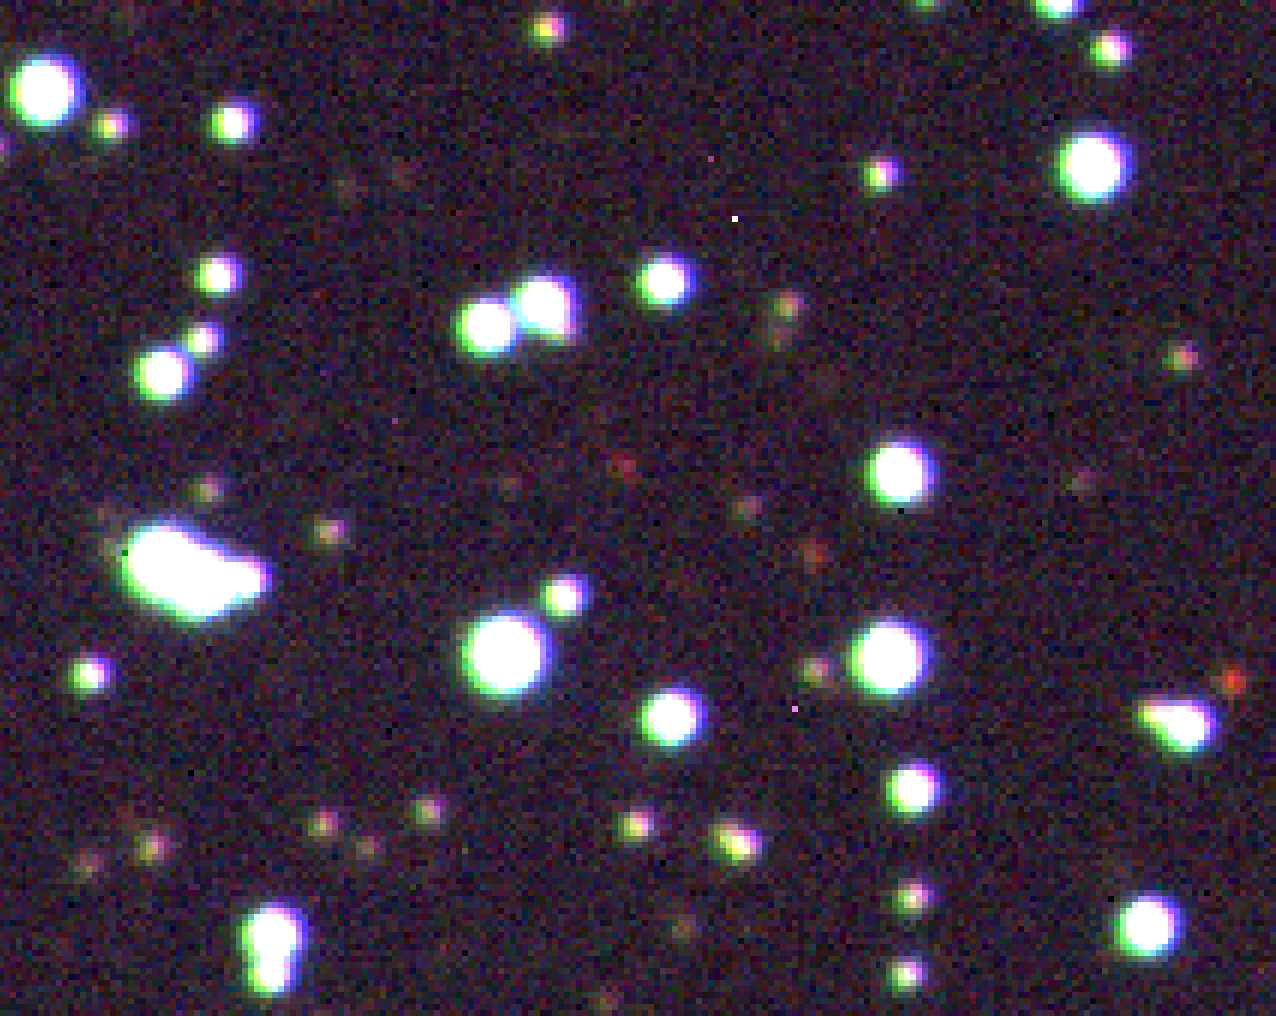
\includegraphics[width=0.5\textwidth]{inventing-color/rgb-bad}
	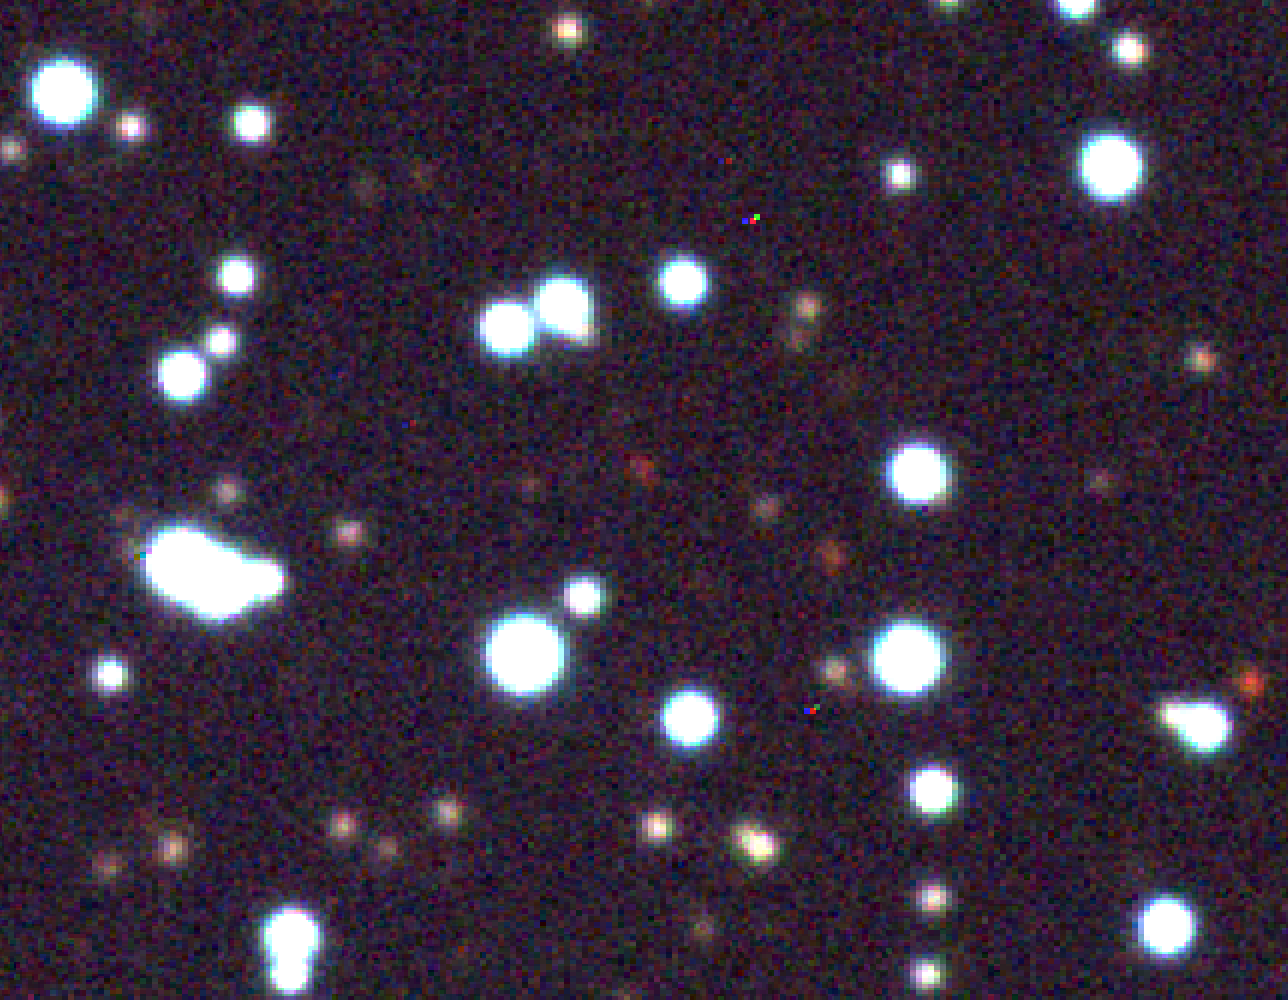
\includegraphics[width=0.5\textwidth]{inventing-color/rgb-good}
	\caption{Zoom-in on a color image, showing poor (left) and good (right) image alignment across filters. Note how objects are shifted between different color channels in the poorly aligned image.}\label{ic:fig:rgb-bad}
\end{figure}